% !TEX root = main.tex

\subsection{博弈树搜索}
% Game tree search: MiniMax, alpha-beta pruning

博弈的一些前提
\begin{itemize}
	\item 两个博弈玩家
	\item 离散值:游戏和决策都可以映射到离散空间
	\item 有限的:只有有限的状态和可能的决策
	\item 零和博弈:完全竞争,即如果一个玩家胜利,则另外一个失去同样数量的收益
	\item 确定性的:没有牵涉到概率性事件,如色子、抛硬币等
	\item 完美信息博弈:状态的所有方面都可以被完全观察,即没有隐藏的卡牌
\end{itemize}

剪刀石头布是简单的一次性(one-shot)博弈
\begin{itemize}
	\item 一次移动
	\item 在博弈论中称为策略或范式博弈(strategic/normal form)
\end{itemize}

但很多游戏是牵涉到多步操作的
\begin{itemize}
	\item 轮回(turn-taking)游戏,如棋类
	\item 在博弈论中称为扩展形式博弈(extensive form)
\end{itemize}

两个玩家$A$(最大化己方收益)和$B$(最小化对方收益)
\begin{itemize}
	\item 状态集合$\mathcal{S}$
	\item 初始状态$I\in\mathcal{S}$
	\item 终止位置$T\subset\mathcal{S}$
	\item 后继:下一可能状态的集合
	\item 效益(utility)/收益(payoff)函数$V:T\mapsto\rr$,表明终止状态对$A$玩家有多好,对$B$玩家有多坏(都站在$A$角度给出)
\end{itemize}

\subsubsection{Minimax策略}
\textemph{自己选max,对方选min}
\begin{itemize}
	\item 构建整棵博弈树,然后将终止/叶子结点标上收益
	\item 回溯整棵树,然后将每个结点都标记上收益
\[U(n)=
\begin{cases}
\min\{U(c):\;c \text{ is a child of } n\} & n \text{ is a Min node}\\
\max\{U(c):\;c \text{ is a child of } n\} & n \text{ is a Max node}
\end{cases}\]
\end{itemize}
\begin{figure}[H]
\centering
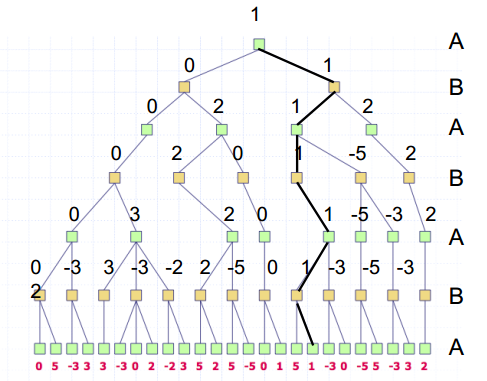
\includegraphics[width=0.6\linewidth]{fig/game-tree.png}
\end{figure}

用DFS可以遍历整棵树,同时保持线性的空间复杂度,每次回溯时更新结点为min/max即可

\subsubsection{Alpha-Beta剪枝}
注意$\alpha$-$\beta$剪枝只要有一祖先大于/小于后代节点的值就可以进行剪枝,即要看\textemph{所有祖先做决定}。
\begin{itemize}
	\item 只要当前Max结点的值$\geq$祖先某一Min结点的值,就可以在该Max结点上做$\alpha$剪枝
	\item 只要当前Min结点的值$\leq$祖先某一Max结点的值,就可以在该Min结点上做$\beta$剪枝
\end{itemize}
即\textemph{当前Min小等祖先Max,当前Max大等祖先Min可剪枝}。
\begin{algorithm}[H]
\caption{Alpha-Beta Pruning}
\begin{algorithmic}[1]
\Procedure{AlphaBeta}{n,Player,alpha,beta}
\If{n is TERMINAL}
\State \Return V(n)\Comment{Return terminal states utility}
\EndIf
\State ChildList = n.Successors(Player)
\If{Player == MAX}
\For{c in ChildList}
\State alpha = max(alpha, AlphaBeta(c,MIN,alpha,beta))
\If{beta <= alpha}
\State break
\EndIf
\EndFor
\State \Return alpha
\Else\Comment{Player == MIN}
\For{c in ChildList}
\State beta = min(beta, AlphaBeta(c,MAX,alpha,beta))
\If{beta <= alpha}
\State break
\EndIf
\EndFor
\State \Return beta
\EndIf
\EndProcedure\Comment{Initial call: AlphaBeta(START-NODE,Player,$-\infty$,$+\infty$)}
\end{algorithmic}
\end{algorithm}

\begin{example}
如下采用$\alpha-\beta$剪枝进行搜索,方形为Max结点,圆形为Min结点。
\begin{figure}[H]
\centering
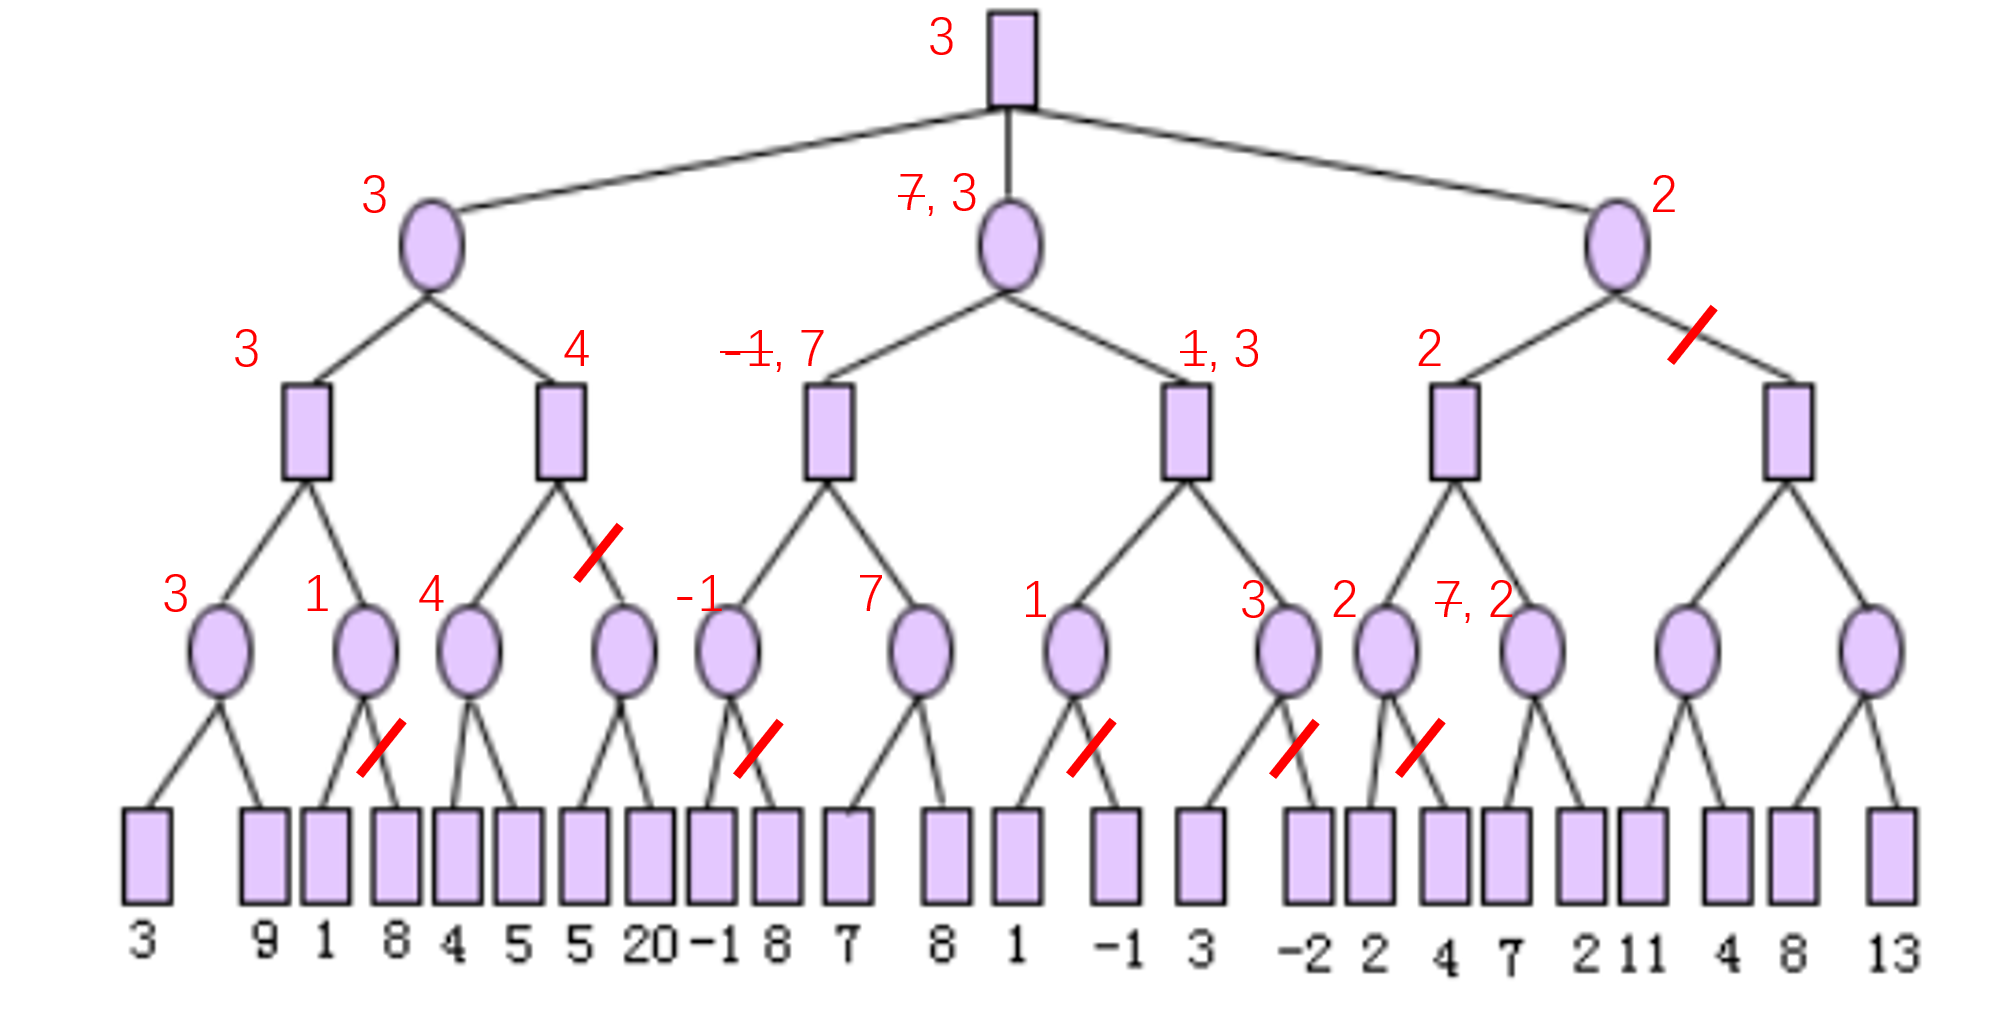
\includegraphics[width=0.9\linewidth]{fig/T01-3.png}
\end{figure}
\end{example}

可以证明,如果原始情况需要访问$O(b^D)$个结点,则经过$\alpha$-$\beta$剪枝后只需访问$O(b^{D/2})$个结点。

\subsubsection{其他补充}
但在现实生活的游戏中,即使采用了$\alpha$-$\beta$剪枝,博弈树也太过庞大。
如棋类的分支因子大致是35,深度为10的树已经到$2.7\times 10^{14}$个结点。
因此不能将整棵博弈树展开,需要采用一些启发式方式进行估计。

评价函数(evaluation)的一些需求:
\begin{itemize}
	\item 对于终止状态,评价函数的序应与真实的收益函数相同
	\item 对于非终止状态,评价函数则应该与真实的胜率相关联
	\item 计算时间不能花太长
	\item 通常取多个特征,然后进行加权求和(先验知识)
\end{itemize}

在线(online)/实时(real-time)搜索
\begin{itemize}
	\item 没有办法展开全部的边界集,因此限制展开的大小(在没找到去目标的真实路径就做出决定/直接选一条路就开始走)
	\item 在这种情况下,评价函数不仅仅引导搜索,更是提交真实的动作
	\item 虽然找不到最优解,但是求解时间大大缩减
\end{itemize}